\numberwithin{equation}{section}

\section{Nondimensionalization}
\begin{frame}
  \frametitle{Outline}
  \tableofcontents[ currentsection ]
\end{frame}

\begin{frame}
\frametitle{Nondimensionalization}

The initial model is:

  \begin{align*}
    \frac{dx}{ds} & = rx \left(1-\frac{x}{k}\right) - \alpha xy, \\
    \frac{dy}{ds} & = \rho y \left(1-\frac{y}{l}\right) - \beta xy.
  \end{align*}
	
Let 
\begin{align*}
		& x \rightarrow A \hat{x} (s) \\
		& y \rightarrow B \hat{y} (s) \\
		& t \rightarrow \tau \cdot s
\end{align*}
When you substitute and group terms the system becomes nondimensionalized. 
\end{frame}

\begin{frame}
The nondimensionalized system is:

	\begin{align*}
		\frac{d{x}}{ds} &= rx(1-x) - \alpha xy, \\
		\frac{d{y}}{ds} &= y(1-y) - \beta xy.
	\end{align*}
\end{frame}


\begin{frame}
\frametitle{Heun's Method}
\begin{itemize}
\item Heun's method is a numerical procedure for approximating ordinary differential equations with a given initial value.
\item First you calculate the intermediate value $\tilde{y}_{i+1}$ and then the final approximation $y_{i+1}$ at the next generation point.
\end{itemize}

\begin{align*}
	\tilde{y}_{i+1} &= y_i + \Delta t \ f(t_i, y_i) \\
	y_{i+1} &= y_i + \frac{\Delta t}{2} \left[f(y_i,t_i) + f(\tilde{y}_{i+1}, t_{i+1})\right]
\end{align*}
\end{frame}


\begin{frame}
   \frametitle{Heun's Method vs. Euler's Method - Simulation}
For the DE $y'=r y$ on $[0,T]$,\\
\vspace{1em}
	\hspace{1.5em} Heun's:$\hspace{1em} \tilde{y}_{i+1} = y_i + \Delta t \ f(t_i, y_i)$ \\
	\hspace{1.5em} Euler's:$\hspace{1em}\tilde{y}_{i+1} = y_i + \Delta t \ f(r, y_i)$ \\
\begin{columns}[t]
    \column{.5\textwidth} 
    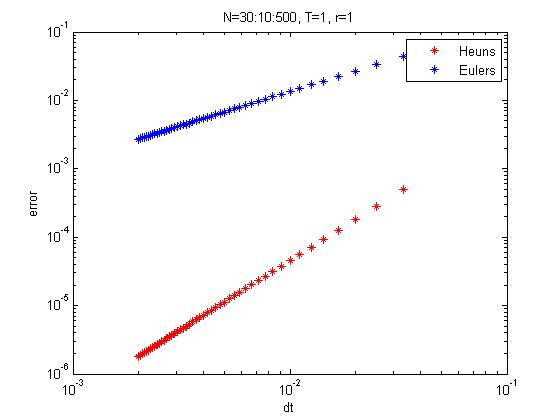
\includegraphics[width=6cm]{img/Heun500}
    \column{.5\textwidth}
    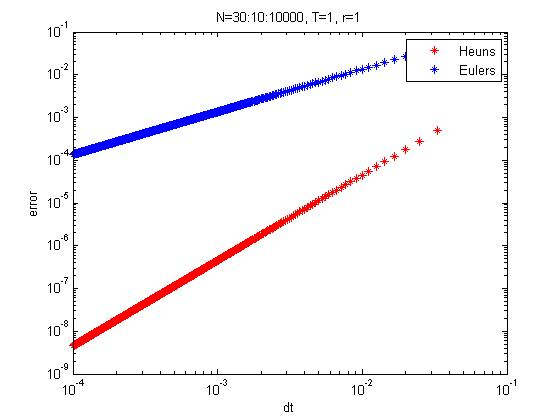
\includegraphics[width=6cm]{img/Heun10000}
  \end{columns}

\end{frame}
